\documentclass{article}

% provides author list facilities
\usepackage{authblk}

% split a float (figure) in independently captioned and labelled sub-regions
\usepackage{subfig}

\usepackage{graphicx}

% hyperlinks in PDF output
\usepackage{hyperref}

% for internal referencing
\usepackage{cleveref}

% to comment out entire blocks
\usepackage{comment}

% \xspace macro to add a "smart" space after a work
\usepackage{xspace}

% allows margin-wise numbering lines
\usepackage[modulo]{lineno}

%-------------------------------------------------------------------------------
%--- the usual endless set of definitions

% software
\newcommand{\PostgreSQL}{PostgreSQL\xspace}
\newcommand{\ART}{\textsl{art}\xspace}
\newcommand{\ARTDAQ}{\textsl{art}DAQ\xspace}
\newcommand{\CLHEP}{CLHEP\xspace}
\newcommand{\ROOT}{ROOT\xspace}
\newcommand{\CRY}{CRY\xspace}
\newcommand{\GENIE}{GENIE\xspace}
\newcommand{\GEANT}{GEANT4\xspace}
\newcommand{\libwda}{\textsl{libwda}\xspace}
\newcommand{\Pandora}{\textsl{pandora}\xspace}
\newcommand{\nutools}{\textsl{nutools}\xspace}
\newcommand{\FHiCL}{FHiCL\xspace}
\newcommand{\UPS}{UPS\xspace}
\newcommand{\cetbuildtools}{\textsl{cetbuildtools}\xspace}
\newcommand{\MRB}{MRB\xspace}
\newcommand{\git}{git\xspace}
\newcommand{\SVN}{SVN\xspace}

\newcommand{\ClassName}[1]{\texttt{#1}}

% experiments
\newcommand{\NOvA}{NO$\nu$A\xspace}

% language
\newcommand{\eg}{e.g.\xspace}
\newcommand{\ie}{i.e.\xspace}

%-------------------------------------------------------------------------------


\begin{document}

\title{The LArSoft architecture (draft)}
% requires authblk

\author[1]{Gianluca~Petrillo}
\author[2]{David~Adams}
\author[3]{Eric~Church}
\author[4]{Amir~Farbin}
\author[1]{Herbert~Greenlee}
\author[1]{Thomas~Junk}
\author[1]{Wesley~Ketchum}
\author[1]{James~Kowalkowski}
\author[1]{Marc~Paterno}
\author[1]{Ruth~Pordes}
\author[1]{Brian~Rebel}
\author[1]{Saba~Sehrish}
\author[1]{Erica~Snider}
\author[5]{Tracy~Usher}
\author[1]{Tingjun~Yang}

\affil[1]{Fermi National Accelerator Laboratory, U.S.A.}
\affil[2]{Brookhaven National Laboratory, U.S.A.}
\affil[3]{Pacific Northwest National Laboratory, U.S.A.}
\affil[4]{University of Texas at Arlington, U.S.A.}
\affil[5]{Stanford Linear Accelerator Laboratory, U.S.A.}

% \author{The LArSoft project}
\maketitle

\linenumbers

\tableofcontents

\section{Introduction}
\label{sec:introduction}

% \section{Introduction}
% \label{sec:introduction}

\subsection{Purpose}
\label{ssec:Introduction:Purpose}

The LArSoft toolkit enables simulation, reconstruction and
physics analysis of data from any detection system based on Liquid Argon TPCs.
Its common tools and algorithms render the development
and analysis process more uniform across the Experiments,
and facilitate direct sharing of code and experience between Experiments.
LArSoft is extensible to accommodate evolving Experiments' needs
and adoption by new Experiments.

This document describes the current architecture of LArSoft toolkit.
The architecture was developed according to, and therefore reflects,
the consensus of LArSoft partners, including the adopting Experiments.

The document provides a reference for the reader interested in learning
the general structure of LArSoft, its functional areas and interactions
with the execution environment.
It also offers guidelines for the contributor aiming to develop new algorithms
within LArSoft or to use it together with external tools.


\subsection{Scope}
\label{ssec:Introduction:Scope}

This document provides an overview of the architecture of LArSoft toolkit,
including its relationship with the surrounding software environment.
The internal flow of the different subsystems is also described.
The document intends to capture and convey the significant architectural decisions,
which reflect into the current implementation or drive its development.\\
Some commonly used LArSoft elements are mentioned to exemplify
flows and connections, but this is no attempt to exhaustively describe
each, or any, of the single elements.

This document describes the architecture of LArSoft to date.
At the time of writing, LArSoft \texttt{v05\_00\_00} is in Release Candidate 2.



\section{Overview}
\label{sec:Overview}

% \section{Overview}
% \label{sec:Overview}

The LArSoft toolkit aims to offer a solution for the typical data analysis scenarios
of an experiment based on a Liquid Argon TPC detector:
\begin{itemize}
  \item generation of physics pseudo-events
  \item simulation of physics processes in the detectors
  \item simulation of the readout response
  \item reconstruction of low and high level physics objects
  \item analysis and presentation of collected data
  \item graphical display of physics events
\end{itemize}

As an example, suppose a scientist may want to develop a new clustering algorithm
optimized for a certain type of physics events.
LArSoft offers interface to generators to produce either simplified physics events
or more realistic ones that include, for example, cosmic radiation.
It also provides the simulation of those events in the specific experiment detector.
If the target processes are common enough, the experiment might have already
executed these steps on large scale, also using LArSoft, and provided the necessary input.
The scientist is then presented with standard interfaces to access geometry and detector
information, and standard data structure to start the reconstruction with,
including single wire hits suitable as starting point for a clustering algorithm,
and to store the results into.
She (or he) can use the standard framework environment to write an algorithm class
and its framework module, compile it and test it immediately on simulated data.
The result, in a standard LArSoft structure, can be immediately visualized in a
event display, and improvement made to the code.
Depending on the algorithm, the time between a code change and the
visualization of its effect may take less than one minute.
Finally, replacing the input with actual detector data, that uses the same format
as the simulation, she will immediately see the performance in the real case.

As a different example, a scientist may want to compare two different algorithms
analyzing reconstructed tracks.
After the tracks are produced, either running the track reconstruction algorithm
on simulated or real data, he (or she) will write one or more analysis algorithms
and their framework modules to produce the necessary plots.

Since LArSoft has been designed to take advantage of the \ART framework\cite{ART},
LArSoft users will extensively work with its concepts,
including for example services and modules, and infrastructure, like \ART scripts
to create skeleton modules, and the configuration based on FHiCL language\cite{FHiCL}.




\section{Logical view: components}
\label{sec:Components}

% \section{Logical view: components}
% \label{sec:Components}

%
% This is the merging of "component view" and "component interafctions"
% from J&M outline, following Saba's suggestion.
%
%

To provide the best solutions for LAr TPC simulation, reconstruction and
analysis of data, LArSoft provides a collection of built in tools and
algorithms, but also interfaces to other existing libraries.
\Cref{fig:LArSoftRelations} illustrates the relation between LArSoft and
these libraries.

\begin{figure}
	\includegraphics[width=\textwidth]{figures/LArSoftArchitectureSimplifiedGraph}
	\caption{\label{fig:LArSoftRelations}
		Relationship between LArSoft and other packages and libraries
	}
\end{figure}

LArSoft is designed to rely on the \ART framework~\cite{ART}.
This framework provides an event data model, centralized configuration, data
and configuration persistency, management of user algorithm through
``modules'', exception handling, and more. LArSoft takes advantage of
the libraries \ART framework depends on, by using them directly:

\begin{itemize}
\item
  FHiCL language~\cite{FHiCL} to propagate the configuration to its
  components
\item
  message facility~\cite{MessageFacility} to regulate text output to console
\item
  CLHEP, ROOT, Boost libraries as needed
\end{itemize}

LArSoft also shares a common platform, \emph{nutools}~\cite{nutools}, with
other neutrino experiments (\NOvA). This library provides LArSoft with
some basic event display facilities and simulation data structures.

LArSoft interactions include:

\begin{itemize}
\item
  experiment detector data, through customized input modules converting
  data into LArSoft data classes
\item
  external event generators (e.g., CRY~\cite{CRY}, GENIE~\cite{GENIE}, via
  API or through HEPEVT exchange format; additional event generators are
  natively implemented in LArSoft
\item
  GEANT~\cite{GEANT}, an external detector simulation library
\item
  data bases, via direct connection or web proxy (\emph{libwda}~\cite{libwda})
\item
  external reconstruction tools (e.g., \emph{pandora}~\cite{pandora}), through a
  LArSoft interface
\item
  custom analysis tools, that can use LArSoft data classes directly or
  tailored data formats produced by custom LArSoft modules
\item
  experiment code, written in the form of LArSoft algorithms, modules
  and services
\end{itemize}




\section{Process view: workflows}
\label{sec:Workflows}

% \section{Process view: workflows}
% \label{sec:Workflows}

LArSoft's tools can be sequenced and combined to compound complete workflows.
The typical usage is aligned to three main types of ``standard'' workflows (\cref{fig:LArSoftProcessingChain}):
\begin{enumerate}
  \item simulation
  \item reconstruction
  \item analysis
\end{enumerate}
where the first step, simulation, is of course skipped when processing real detector data.
\begin{figure}[htbp]
  \centering
  \includegraphics[width=\textwidth]{figures/LArSoftWorkflows.pdf}
  \caption{\label{fig:LArSoftProcessingChain}Typical workflow sequence in liquid argon TPC analysis. Each block represents a workflow.}
\end{figure}
LArSoft does not directly define these processing chains.
Rather, it inherits the flexibility from the \emph{art} framework,
which provides users with the flexibility of choosing and arranging
processing modules at will. %, with the only limitation that each module
% must be provided with all the information it needs to operate.
A module can also be executed multiple times, with different configurations.\\
Thus, the Experiments define the steps of each workflow according to their
needs.
Still, these needs are fairly shared,
and it is possible to characterize a ``typical'' chain for each workflow.


\subsection{Simulation workflow}
\label{ssec:Workflows:Simulation}

The purpose of a simulation workflow is to describe a realistic response of
the detectors to a known physics event (``truth'').
Since the result of the simulation should be equivalent to the output of the detectors,
this result is represented by the same data classes.

The main results of this workflow are:
\begin{itemize}
	\item data products representing the detector response (\eg \ClassName{raw::RawDigit} and \ClassName{raw::OpDetWaveform})
	\item data products representing the simulated physics (\eg \ClassName{simb::MCTruth}, \ClassName{simb::MCParticle}
\end{itemize}

\begin{figure}[htbp]
  \centering
  \includegraphics[width=\textwidth]{figures/LArSoftSimulationGraph.pdf}
  \caption{\label{fig:LArSoftSimulation}A typical LArSoft simulation workflow.}
\end{figure}
The complete simulation chain is summarized in \cref{fig:LArSoftSimulation}.
The process is typically divided in three steps:
\begin{enumerate}
  \item event generation
  \item detector physics simulation
  \item detector readout simulation
\end{enumerate}

The physics event can be generated by an external program or library.
LArSoft currently interfaces directly to GENIE generator (neutrino interactions)
and CRY (cosmic rays). It can also read a generic HEPEVT\cite{HEPEVT} format.
In addition, LArSoft provides built-in generators to simulate single particles,
Argon nucleus decays, and more.

The detector physics simulation includes the interaction of the
generated particles with the detector, and the propagation to the
readout of produced photons and electrons. This part of the simulation
relies on GEANT4 for the interaction of particles with matter. Photon
and electron transportation to the readout are implemented in built-in
code. Detector parameters (\eg, the intensity of the electric field)
can be acquired from the job configuration or from a custom data base.

The last step transforms the physics information, electrons and photons,
into digitized detector response, including the simulation of
electronics noise and shaping. This is typically implemented with
experiment-specific code.


\subsection{Reconstruction workflow}
\label{ssec:Workflows:Reconstruction}

The reconstruction phase produces standard physics objects to describe
the physics event. Reconstruction delivers objects with different level
of sophistication and from different steps, as for example hits
describing localized charge deposition as detected on a wire, down to a
complete hierarchy of three-dimensional tracks. These objects are handed
over for further analysis.
\begin{figure}[htbp]
  \centering
  \includegraphics[width=\textwidth]{figures/LArSoftReconstructionGraph.pdf}
  \caption{\label{fig:LArSoftReconstruction}A typical LArSoft reconstruction flow.}
\end{figure}
Through the workflow, detector and data acquisition parameters
can be acquired from Experiment data bases.

Starting from detector response, either real or simulated, there are
many possible patterns of analysis. The more ``traditional'' one \cref{fig:LArSoftReconstruction}) proceeds through:
\begin{enumerate}
  \item calibration of the signals, noise suppression and removal of electronics distortions;
  \item independent reconstruction of charge deposition on each TPC wire (\emph{hits});
  \item definition of \emph{clusters} from hits lying on the same wire plane;
  \item combination of clusters from different planes in trajectories (\emph{tracks}) and particle cascades (\emph{showers});
  \item identification of interaction points (\emph{vertices});
  \item hierarchal connection of them into \emph{particle flow} structures. Many options are implemented in LArSoft for each.
\end{enumerate}
Different algorithms can be chosen to perform each of these steps.
Any external library that utilizes LArSoft data classes to receive
inputs and deliver results is also fully interchangeable with the
algorithms implemented in LArSoft. A noticeable example is the
\emph{pandora} pattern recognition toolkit, that accepts LArSoft hits as
input and can present its results in the form of LArSoft clusters,
tracks and particle flow objects.

Alternative workflows can and have been developed.
For example, a derivation of the workflow described above consists in a complete
first pass tuned to the reconstruction and subsequent identification of background
objects (mostly cosmic rays), in their elimination at the level of hits,
and a second pass tuned for reconstruction of neutrino interactions.

Other approaches include direct track reconstruction without clustering,
direct clustering from calibrated or uncalibrated channel signals
by image processing algorithms, bypassing the construction of hits, and more.

LArSoft and \ART modularity allows to arrange for acyclic workflows
with any predetermined number of (potentially optional) steps.
It does not accommodate cyclic workflows.


\subsection{Analysis workflow}
\label{ssec:Workflows:Analysis}

Analysis workflows are the most vaguely defined,
due in part to the more diverse goals,
and partly to the fact that in this relatively early stage the Experiments
have devoted most of the time to simulation and reconstruction.

The calibration of energy deposited in liquid argon by interacting particles
and their identification as specific types (\eg, muons, protons, etc.)
have been classified sometimes as ``analysis'', sometimes as ``reconstruction''.
Another common analysis task is evaluation of reconstruction performances
and comparison between different algorithms and strategies.

Calibration activities, for example pedestal analysis,
characterization of argon purity, mapping of the electric field,
also fall in this category and they are ideal candidates for the standardization of workflows.




\section{Deployment view: development and extensibility}
\label{sec:Development}

% \section{Deployment view: development and extensibility}
% \label{sec:Development}

The extensibility of LArSoft is largely based on the underlying
framework, \ART. The \ART framework processes physics \emph{event}
independently, executing on each of them a sequence of \emph{modules}.
An event is defined by an input module.
In most Experiments it is bound to a single pulsed beam interaction with the detector,
but test beam Experiments, non-beam Experiments and non-beam analyses (\eg proton decay)
may need to define different event boundaries.
The framework also provides a list of global \emph{services} that modules can rely on.
Examples of services implemented by LArSoft include
the description of detector geometry and channel mapping,
the set of detector configuration parameters,
and access to TPC channel quality information.

In this section we describe the development environment
and then focus on the main handles LArSoft offers developers for the sake of extensibility,
including new serializable data structures, new algorithms
and the use of external libraries.


\subsection{Development environment}
\label{ssec:Development:Environment}

LArSoft is designed for and supports the use of a development environment based on:
\begin{itemize}
   \item UNIX Product Support (\UPS) for access to dependent packages
   \item \cetbuildtools\cite{cetbuildtools} as build system
   \item Multi-Repository Build\cite{MRB} (\MRB)  to coordinate build and execute software from different repositories
   \item \git (recommended) or \SVN for version control
\end{itemize}
The following description assumes the prerequisite availability of all these tools.

LArSoft is fully supported on the following platforms:
\begin{itemize}
   \item Scientific Linux Fermi: version 6
   \item Darwin: version 13 (OS X 10.9 ``Maverick'') and 14 (OS X 10.10 ``Yosemite'')
\end{itemize}
LArSoft typically supports the two most recent versions of these operating systems\footnote{
The actual supported versions depend also on the underlying support of the O.S. by Fermilab.
}.
Support is also planned for the long term support release of Ubuntu Linux (16.04 LTS).

A typical workflow starts with the set up of a working area.
After the area is created the first time, subsequent utilization of it requires just a simple set up.
LArSoft provides a script for this set up,
and it is common practice for the Experiments to provide customized ones.

The development, whether it is creation of new code or modification of existing one,
follows the following workflow:
\begin{enumerate}
   \item \emph{development-specific set up} of the existing working area
   \item importing the source code to be modified, if any; this code will persist in the area
   \item modifications as needed
   \item building
   \item optional (and recommended) execution of a standard test suite
   \item installation for running
\end{enumerate}

The execution of LArSoft code including user development, as described above,
follows this workflow:
\begin{enumerate}
   \item \emph{run-time specific set up} of the existing working area
   \item preparation of job configuration as needed
   \item execution of the software
\end{enumerate}
The execution of LArSoft code as distributed, without modification,
has a simpler set up that does not require a development working area.\\
LArSoft and the Experiments provide a vast selection of configurations ready to run, making the second step optional.
Development and execution set up can coexist in the same environment at the same time.

LArSoft currently provides no facility to execute code remotely,
including job submission to remote clusters.
The Experiments supply workflows and scripts for this type of execution.



\subsection{Testing}
\label{ssec:Development:testing}

LArSoft development model allows multiple contributors to modify the
code at the same time. This model can create conflicts and dysfunction
in the code. Tests are instrumental to the early detection of such
defects. LArSoft includes tests at two levels, called \emph{unit tests}
and \emph{integration tests}.

Unit tests exercise a limited part of the system, typically a single algorithm.
Ideally a unit test for an algorithm should test all the functions of that algorithm.
In practice, tests for complex algorithms tend to set up and test a few known typical cases.
Unit tests can be added at the same time the tested code is beging developed.
They are run in the development environment:
as such, they are the quickest mean to exercise newly written code.

Integration tests involve the framework and one or more processing modules.
These tests can reproduce real user scenarios,
for example a part of the official processing chain of an Experiment,
and they can compare new and historical results.
LArSoft tools allow these tests to be run on demand at any time,
and a standard suite of tests is automatically and periodically run
as part of LArSoft Continuous Integration system.


\subsection{Data products}
\label{ssec:Development:DataProducts}

LArSoft provides a basic set of serializable data classes.
Each class is associated to a simple concept and a set of related quantities.
For example, \texttt{raw::RawDigit} describes the raw data as read from a TPC channel;
\texttt{recob::Cluster} describes a set of correlated hits observed on a wire plane;
\texttt{anab::Calorimetry} contains information about calibrated energy of a track.

A \emph{data product} is a class that:
\begin{itemize}
   \item is simple: contains just data and trivial logic to access it;
      more complex elaborations belong to algorithms
   \item contains only members from a small set of selected libraries:
      C++ standard library is highly recommended; ROOT classes are also accepted
   \item is not polymorphic
\end{itemize}

Limitations to ROOT I/O system impose restrictions on the types of allowed data members,
\eg on the set of supported C++11 containers.
Relations between data products are expressed by \emph{associations}.
Associations are data products provided by \ART
which can relate a data product, or an element of it,
to another element from another data product.
Examples of use in LArSoft include associations between a
reconstructed hit and the calibrated signal it's reconstructed from, and
between a cluster and all the hits that constitute it.

Data products have a fundamental structural role:
they act as messages to be exchanged between algorithms.
As such, they are also the format in which most of the results are saved.
This allows to arbitrary split the processing chain in multiple sequences of jobs.


\subsection{User code}
\label{ssec:Development:UserCode}

Algorithms constitute, together with data products, the heart of LArSoft,
and the ability for the users to add their own algorithm is central to its design.
In fact, LArSoft algorithms differ from users' algorithms
only in the consideration that their purpose is of general interest.
Indeed, most of the algorithms in LArSoft were written by users to solve their own specific problems,
and then adopted into the common toolkit.
LArSoft encourages users to produce algorithms that perform correctly on \emph{any} liquid argon detector,
and to integrate them into LArSoft itself.

\begin{figure}
   \centering
   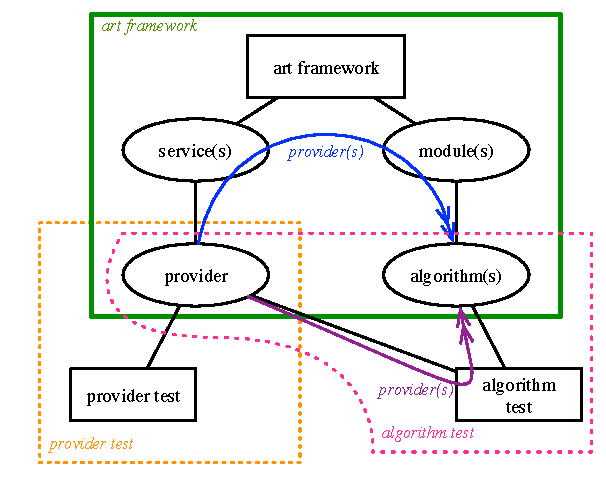
\includegraphics{figures/LArSoftFactorizationModelAndTests}
   \caption[LArSoft algorithm and service model]{
      \label{fig:AlgorithmModel}
      LArSoft algorithm and service model.
      Black lines represent ownership.
      The coloured arrows show the path the algorithm obtains the provider through.
      The green line contours the standard execution environment.
      Dotted lines describe testing environments:
      both service providers and algorithms can be tested without involving the full framework.
   }
\end{figure}

The preferred model for algorithm design is represented in \cref{fig:AlgorithmModel}.
We refer to this as \emph{factorization} model.
The underlying principle it is that the algorithm must be independently
testable and portable, using the minimal set of necessary dependences.
This also allows for the algorithms to be used in contexts where the
\ART framework is not available,
provided that some other system supplies equivalent functionalities as,
and only when, needed. The model is made of two layers:
\begin{enumerate}
   \item
      the algorithm, in the form of a class that
      \begin{itemize}
         \item
            is configurable with FHiCL parameter sets
         \item
            consumes LArSoft data products as input
         \item
            produces LArSoft data products as output
         \item
            has the minimal convenient set of dependencies
         \item
            elaborates a single event or part of an event at a time
      \end{itemize}
   \item
      a module for the \ART framework, that:
      \begin{itemize}
         \item
           owns and manages the lifetime of one or more algorithm classes
         \item
           provides the algorithm(s) with the configuration, the data products
           and the information it needs to operate
         \item
           delivers algorithm output to the \ART framework
      \end{itemize}
\end{enumerate}

Since algorithms often rely on services, the services also need to
follow the same factorization model and be split in:

\begin{enumerate}
   \item
      a \emph{service provider}, in the form of a class that:
      \begin{itemize}
         \item
            is configurable with FHiCL parameter sets
         \item
            has the minimal convenient set of dependencies
         \item
            provides actual functionality
      \end{itemize}
   \item
      a service for the \ART framework, that:
      \begin{itemize}
         \item
            owns and manages the lifetime of its service provider
         \item
            provides modules with a pointer to the provider
         \item
            when relevant, reacts to messages from the framework (e.g., the
            beginning of a new run) and propagates them to the provider as needed
      \end{itemize}
\end{enumerate}
The module is also responsible of communicating to its algorithms which
service providers to use. Algorithms exclusively interact with service
providers rather than with \ART services.

Other important guidelines for the development of algorithms are:

\begin{description}
   \item[interoperability]
      they should document their assumptions in detail,
      and correctly perform on any detector if possible
   \item[modularity]
      each algorithm should perform a single task;
      complex tasks can be performed by hierarchies of algorithms
   \item[maintainability]
      they should come with complete documentation and proper tests
\end{description}

\Cref{fig:AlgorithmModel} shows that if algorithms are not
framework-dependent, their unit test can also be framework-independent.
Therefore, not only those algorithms can be developed in a simplified,
framework-unaware environment, but they can also be tested in that same
development environment. In other words, the full development cycle, of
which testing is an integral part, can seamlessly happen in the same
environment.


\subsection{External libraries}
\label{ssec:Development:ExternalLibraries}

We call ``external'' any library that does not depend on LArSoft, with
the possible exception of its data products. Examples in this category
are \GENIE, \GEANT, and \Pandora.

LArSoft's modularity can accommodate contributions from external
libraries into its workflow (\cref{fig:LArSoftAndExternals}). The
preferred way is to use directly the external library via its interface.
This requires an additional interface module between LArSoft and the
library, in charge of converting the LArSoft data products into a format
digestible by the external library, configuring and driving it, and
extracting and converting the results into a set of LArSoft data
products.
\begin{figure}
   \centering
   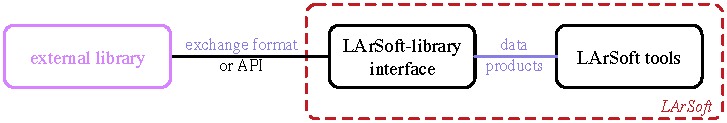
\includegraphics{figures/LArSoftAndExternalLibrary}
   \caption[Interaction between LArSoft and an external library]{
      \label{fig:LArSoftAndExternals}
      Interaction between LArSoft and an external library.
      The dashed line encompasses the components belonging to LArSoft.
      Shapes and colours are as in \cref{fig:LArSoftSimulationRelations}.
   }
\end{figure}

This model is exemplified in the interaction between LArSoft and
\Pandora\cite{pandora} (\cref{fig:LArSoftAndPandora}): \Pandora uses
its own data classes for input hits, particle flow results and geometry
specification. A base module exists that reads LArSoft hits, converts
them into \Pandora's, translates geometry information,
and LArSoft clusters, tracks, vertices, and more,
out of \Pandora particle flow objects.
\begin{figure}
   \centering
   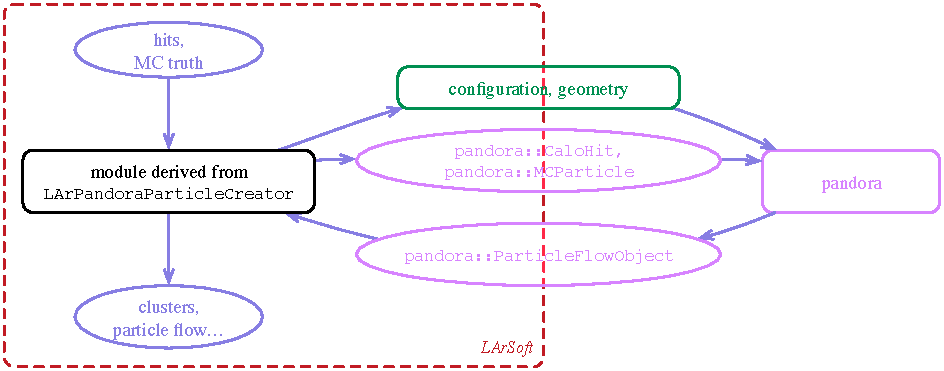
\includegraphics{figures/LArSoftAndPandora}
   \caption[Model of communication between LArSoft and \Pandora]{
      \label{fig:LArSoftAndPandora}
      LArSoft workflow including \Pandora.
      Data structures in the \texttt{pandora} namespace are defined in \Pandora
      and also known by LArSoft.
   }
\end{figure}\\
This approach has relevant advantages: it can be fairly fast; it allows
a precise translation of information; it provides the greatest control
on the flow within the library; it defines and tracks the configuration
of the external library. Its greatest drawback is the need for the
LArSoft interface to depend on the external library. If this limitation
is not acceptable, a more independent communication channel can be
established via exchange files. In this case, LArSoft interface
translates data products into a neutral format, possibly based solely on
ROOT objects or on a textual representation, and back into data
products. The external library is in charge of performing the equivalent
operations with the library data format. This is for example the generic
communication mechanism with event generators that support HEPEVT
format. The strong decoupling comes at the price of a fragmented
execution chain and the burden of additional configuration consistency
control, for example to ensure that a consistent geometry was used for
the information (re)entering LArSoft.



\section{Physical view: repositories and packages}
\label{sec:Packages}

% \section{Deployment view: repositories and packages}
% \label{sec:Repositories}

LArSoft supports the use of the UNIX Product Support (\UPS) system
for deployment of LArSoft itself and of the additional software it depends from.
This system is organized in \emph{products} containing executable code for a specific platform
and auxiliary data as needed.
LArSoft set up demands from UPS a specific version of almost every library LArSoft depends on,
including for example the GNU compiler, Boost libraries and CERN ROOT.

LArSoft code base is organized in \emph{repositories} grouping different functionalities.
The current list of repositories is:
\begin{description}
   \item[larcore] independent of data products (\eg geometry description)
   \item[lardata] defining the shared data products
   \item[larevt] code independent of simulation and reconstruction algorithms (\eg calibration, database access)
   \item[larsim] detector simulation
   \item[larreco] physics object reconstruction
   \item[larana] depending on simulation or reconstruction algorithms (\eg particle identification, calorimetry)
   \item[larpandora] interface with pattern recognition package \Pandora
   \item[lareventdisplay] ROOT-based visualization tool
   \item[larexample] examples of LArSoft modules
   \item[larsoft] ``umbrella'' product
\end{description}
Additional LArSoft repositories do not contain source code:
\begin{description}
   \item[larsoft\_data] containing small-size, slowly-changing data files
   \item[lar\_ci] providing a Continuous Integration test system that allows instant, thorough test of the code
\end{description}

LArSoft repositories are maintained in Fermilab Redmine as \git repositories.


\subsection{Local LArSoft installation}
\label{ssec:Repositories:LocalInstallation}

LArSoft can be installed in any supported platform, either with:
\begin{description}
   \item[binary installation] copying prebuilt UPS products from Fermilab server
      into a local UPS directory
   \item[source installation] copying, building and installing into a local UPS directory
      the source code of each and every dependent package
\end{description}
Both installation patterns are supported via a single script.
In this way, LArSoft can be installed in virtual machines, personal computers
as well as in computing clusters.


%%%%%%%%%%%%%%%%%%%%%%%%%%%%%%%%%%%%%%%%%%%%%%%%%%%%%%%%%%%%%%%%%%%%%%%%%%%%%%%%
%%% References


% the order of references is determined by the order of \cite and \nocite commands
\bibliographystyle{unsrt}

\bibliography{sources/references}



%%%%%%%%%%%%%%%%%%%%%%%%%%%%%%%%%%%%%%%%%%%%%%%%%%%%%%%%%%%%%%%%%%%%%%%%%%%%%%%%

\clearpage
\appendix

%%%%%%%%%%%%%%%%%%%%%%%%%%%%%%%%%%%%%%%%%%%%%%%%%%%%%%%%%%%%%%%%%%%%%%%%%%%%%%%%

\section*{Comments}
\label{sec:comments}

% \section*{Comments}
% \label{comments}


\subsection*{\texorpdfstring{Sunday 7:51:39, Ruth Pordes
\href{mailto:ruth@fnal.gov}{\nolinkurl{ruth@fnal.gov}} (``Re: First
draft of the architecture description
document'')}{Sunday 7:51:39, Ruth Pordes ruth@fnal.gov (``Re: First draft of the architecture description document'')}}\label{sunday-75139-ruth-pordes-ruthfnal.gov-re-first-draft-of-the-architecture-description-document}

\emph{{[}Q 001{]}} does the scope include human interfaces as well as
software?\\
\emph{{[}A 001.1{]}} \emph{{[}GP{]}} I thought mostly not, but I am not
completely sure what human interface includes. To be clarified.
\emph{(TODO)}

\emph{{[}Q 002{]}} nutools event display facility and simulation data
structures -- still does not make sense to me. Is Visualization one
special kind of analysis or does Larsoft have specific interfaces to
it?\\
\emph{{[}A 002.1{]}} \emph{{[}GP{]}} Visualization is a special kind of
analysis. But our event display crosses the border with its (limited)
ability to \emph{interactively} reprocess the input.

\emph{{[}Q 003{]}} page 4 -- can components of the chain be re-executed
during a single pass?-\\
\emph{{[}A 003.1{]}} \emph{{[}GP{]}} I have added a couple of sentences
in the previous-to-last paragraph of Architecture \textgreater{}
Overview section, that I hope give an answer. The answer is very much in
the features of art, that I have not covered at all in this text. Should
we? \emph{(TODO)}

\emph{{[}Q 004{]}} does event display have a specific meaning - I'll
include it in the Requirements glossary -- it is different from a
generalized visualization and I presume the definition should explain
this? Also, if the event display is in nutools it is not part of
larsoft??? Can we share a glossary in some fashion?\\
\emph{{[}A 004.1{]}} \emph{{[}GP{]}}

\emph{{[}Q 005{]}} Figure 2. You explicitly mean Detector not DAQ ?
Does/shoud daq show up somewhere\\
\emph{{[}A 005.1{]}} \emph{{[}GP{]}} in practice DAQ products is what we
communicate with. It doesn't have to be only that, but I guess that is
it effectively what happens. \emph{(TODO)}

\emph{{[}Q 006{]}} a Fluka interface is in the works with integration
hoped for before the end of Dec. Can you include a sentence on this
interface?\\
\emph{{[}A 006.1{]}} \emph{{[}GP{]}} Erica, confirm? \emph{(TODO)}

\emph{{[}Q 007{]}} page 10.Unit test. These are important. These are not
the only tests. I don't see them referred to and perhaps some more
specifics might be useful?\\
\emph{{[}A 007.1{]}} \emph{{[}GP{]}} I added a section about testing. I
have added a few words also at the point Ruth specified (at the end of
``User code'' section). I think it would be good to add a ``test'' block
in one of the high-level diagrams, but I can't figure out where. Or maybe we
have to add a \emph{development model} section?




\end{document}
